\documentclass[11pt,a4paper]{article}
\usepackage[utf8]{inputenc}
\usepackage[T1]{fontenc}
\usepackage{lmodern}
\usepackage[margin=2.5cm]{geometry}
\usepackage{amsmath,amssymb}
\usepackage{booktabs}
\usepackage{graphicx}
\usepackage{hyperref}
\usepackage{xurl}
\usepackage{setspace}
\onehalfspacing

\hypersetup{
    colorlinks=true,
    linkcolor=blue,
    citecolor=blue,
    urlcolor=blue
}

\title{\textbf{Eurasian Continental Bridges: Silver Living Costs, Internal Russian Convergence, and the Great Divergence, 1738--1913}}

\author{Petr Avtonomov\thanks{Independent Researcher, St.~Petersburg, Russia. ORCID: \url{https://orcid.org}. Code and data repository: \url{https://github.com/avtonomov-petr/Eurosean-Continental-Bridges}.}}
\date{November 2026}

\begin{document}

\maketitle

\begin{abstract}
Building on three companion audits of Atlantic grain prices (\href{https://doi.org}{Avtonomov, 2026a}), Baltic Sound Toll shipping (\href{https://doi.org}{Avtonomov, 2026b}), and St.~Petersburg--European exchange rates (\href{https://doi.org}{Avtonomov, 2026c}), this paper extends the diagnostic framework across the Eurasian landmass from Western Europe through Imperial Russia to Qing China over \texttt{1738--1913} ($T = 176$ years). Combining pure silver barebones consumer price indices (CPI) and welfare ratios from Allen et al.\ (2011) for \texttt{London}, \texttt{Amsterdam}, \texttt{Leipzig}, \texttt{Florence}, \texttt{Beijing}, \texttt{Suzhou}, and \texttt{Canton} with Russian regional silver wheat series (Mironov, 2010) and benchmark Moscow silver subsistence baskets (Korchmina, 2025), we audit internal Russian convergence alongside the Eurasian Great Divergence. In the 1740s, living costs across Eurasia inhabited a narrow metallic band (157--208\,g of pure silver per person-year), while Moscow stood roughly half as expensive (100.1\,g in the 1760s) before converging upward toward Amsterdam and Beijing by the 1780s (224.4\,g). Evaluating the strictly uninterpolated seven-city panel over \texttt{1739--1833} ($M = 95$, zero missing values) confirms a persistent tri-polar geography even prior to the Opium Wars: the Western/Central European core (\texttt{Amsterdam} $v_1 = +0.553$, \texttt{London} $+0.464$, \texttt{Leipzig} $+0.357$), maritime southern China (\texttt{Canton} $-0.436$, \texttt{Suzhou} $-0.298$), and isolated continental \texttt{Beijing} ($v_1 = +0.066$; $\mathrm{Mode~2} = +0.451$). After 1840, the four unbroken European cities coalesced into a symmetric co-moving monolith ($\mathrm{Var}_1 = 59.2\%$; individual shares 21.2--28.7\%), whereas \texttt{Beijing} detached almost completely (Mode~1 share falling from 3.97\% in 1739--1839 to 0.97\% in 1840--1913; $v_{2,\mathrm{Beijing}} = -0.971$). Non-parametric transition-graph scanning reveals a two-stage divergence: real living standards (\emph{welfare ratios}) fractured first in \texttt{1857} ($p < 0.0001$) amid the Taiping Rebellion and mid-century industrial crises, whereas silver-denominated price levels (\emph{CPI}) broke decisively in \texttt{1891} ($p = 0.0084$ for $N=5$; $p = 0.0008$ for $N=7$) during global silver demonetization.
\end{abstract}

\noindent\textbf{Keywords:} economic history, Great Divergence, Eurasian trade, Qing China, Russian Empire, silver prices, living standards, Kyakhta trade, cliometrics, spectral analysis.

\section{Introduction}

In three preceding studies of early modern market integration, we traced how Europe and Imperial Russia connected across commodity prices (\href{https://doi.org}{Avtonomov, 2026a}), Baltic maritime shipping (\href{https://doi.org}{Avtonomov, 2026b}), and foreign exchange markets (\href{https://doi.org}{Avtonomov, 2026c}). Yet Imperial Russia was never solely a Baltic-facing maritime power: its eastern frontier stretched across the Urals and Siberia through Lake Baikal and the Buryat border town of Kyakhta directly into northern Qing China (Foust, 1969; Sladkovskii, 1974; Mironov, 2010).

In the broader cliometric debate on the Great Divergence (Pomeranz, 2000; Allen et al., 2011; Broadberry et al., 2018), scholars have extensively compared real wages and living costs at the two maritime extremes of Eurasia—Northwestern Europe versus the Lower Yangzi delta and Canton—while paying less quantitative attention to the continental interior linking Moscow, St.~Petersburg, Siberia, and Beijing. This study bridges that gap by combining unbroken annual silver price and welfare-ratio series for Western Europe and Qing China (\texttt{1738--1913}, $T = 176$ years) with regional silver wheat prices across European Russia (\texttt{1720s--1800s}) and benchmark Moscow silver subsistence baskets (\texttt{1738--1859}).

We establish three empirical findings:
\begin{enumerate}
    \item \textbf{Internal Russian Convergence and Mid-Eurasian Positioning:} During the mid-eighteenth century, Moscow's silver subsistence cost (100.1\,g Ag/year in the 1760s) stood well below both Western Europe (190--238\,g) and Qing China (191--219\,g). Between the 1750s and 1800s, regional silver wheat prices across Novgorod--St.~Petersburg, Moscow, and the Northern Dvina (Arkhangelsk) converged upward into the 0.60--0.71\,g Ag/kg range, lifting Moscow's silver living costs into parity with Amsterdam and Beijing by the 1780s (224.4\,g).
    \item \textbf{Pre-Opium War Tri-Polarity and Post-1840 European Consolidation:} Evaluating the strictly uninterpolated seven-city panel over \texttt{1739--1833} ($M = 95$ transitions, zero missing observations) demonstrates that Eurasia was already divided into three distinct price regimes before the Opium Wars: the European core (\texttt{Amsterdam}, \texttt{London}, \texttt{Leipzig}, \texttt{Florence}), maritime southern China (\texttt{Canton}, \texttt{Suzhou}), and continental northern China (\texttt{Beijing}, the southern terminus of the overland Kyakhta caravan route). After 1840, the four unbroken European cities synchronized into a nearly uniform co-moving block ($\mathrm{Var}_1 = 59.2\%$), while \texttt{Beijing} detached almost completely (Mode~1 share dropping from 3.97\% to 0.97\%; $v_{2,\mathrm{Beijing}} = -0.971$).
    \item \textbf{Two-Stage Eurasian Structural Break (1857 in Welfare Ratios vs.\ 1891 in Silver Prices):} Spectral transition-graph scanning reveals that real living standards (\emph{welfare ratios}) fractured first in \texttt{1857} ($p < 0.0001$), coinciding with the Taiping Rebellion, the Second Opium War, and European industrial divergence, whereas silver-denominated price indices (\emph{CPI}) experienced a sharp regime break in \texttt{1891} ($p = 0.0084$ for $N=5$; $p = 0.0008$ for $N=7$), when global silver demonetization separated gold-standard Europe from silver-standard China.
\end{enumerate}

\section{Data Architecture and Metallic Standardization}

To ensure strict cross-continental comparability without exchange-rate distortion, all price and living-standard series are standardized in grams of pure silver:
\begin{itemize}
    \item \textbf{Eurasian Annual Barebones CPI and Welfare Ratios (1738--1913):} Drawn from Allen et al.\ (2011) via the Global Price and Income History Group (GPIHG), providing annual barebones subsistence basket costs (in grams of pure silver per person-year) and real welfare ratios for \texttt{London}, \texttt{Amsterdam} (1738--1910, linearly bridged for 1911--1913), \texttt{Leipzig}, \texttt{Florence/Milan}, and \texttt{Beijing} (176/176 consecutive CPI observations; 153/176 welfare-ratio observations for Beijing). For maritime southern China, \texttt{Suzhou} (100 observations) and \texttt{Canton} (103 observations) form a continuous, zero-missing series from 1738 through 1833 before reporting gaps during the Opium War and Taiping eras (resuming in 1910--1913). Accordingly, we evaluate both the strictly uninterpolated seven-city panel over \texttt{1739--1833} ($M = 95$) and the bridged 1739--1913 panel ($M = 175$) alongside the unbroken five-city core.
    \item \textbf{Moscow Silver Baskets and Regional Russian Grain Series:} Drawn from Korchmina (2025) for Moscow barebones subsistence baskets in grams of pure silver (33 benchmark years across 1738--1859 where full non-grain components—beef, butter, salt, tallow candles, linen, soap, and firewood—are simultaneously documented alongside rye) and Mironov's (2010) decadal regional wheat prices (grams of silver per kilogram) across \texttt{Novgorod--St.~Petersburg}, \texttt{Moscow}, and \texttt{North Dvina (Arkhangelsk)} over 1720s--1800s.
\end{itemize}

\section{Empirical Results}

\subsection{Internal Russian Convergence and Mid-Eurasian Silver Levels}
Comparing decadal averages across the Eurasian landmass highlights how Imperial Russia bridged the gap between low-cost interior agriculture and high-silver-price maritime hubs (Figure~\ref{fig:fig1}A--B). In the 1740s, barebones living costs across \texttt{London} (208.3\,g Ag/year), \texttt{Amsterdam} (181.4\,g), \texttt{Florence} (180.0\,g), \texttt{Leipzig} (161.4\,g), \texttt{Beijing} (171.2\,g), \texttt{Suzhou} (190.5\,g), and \texttt{Canton} (156.9\,g) occupied a compact silver band.

\begin{figure}[htbp]
\centering
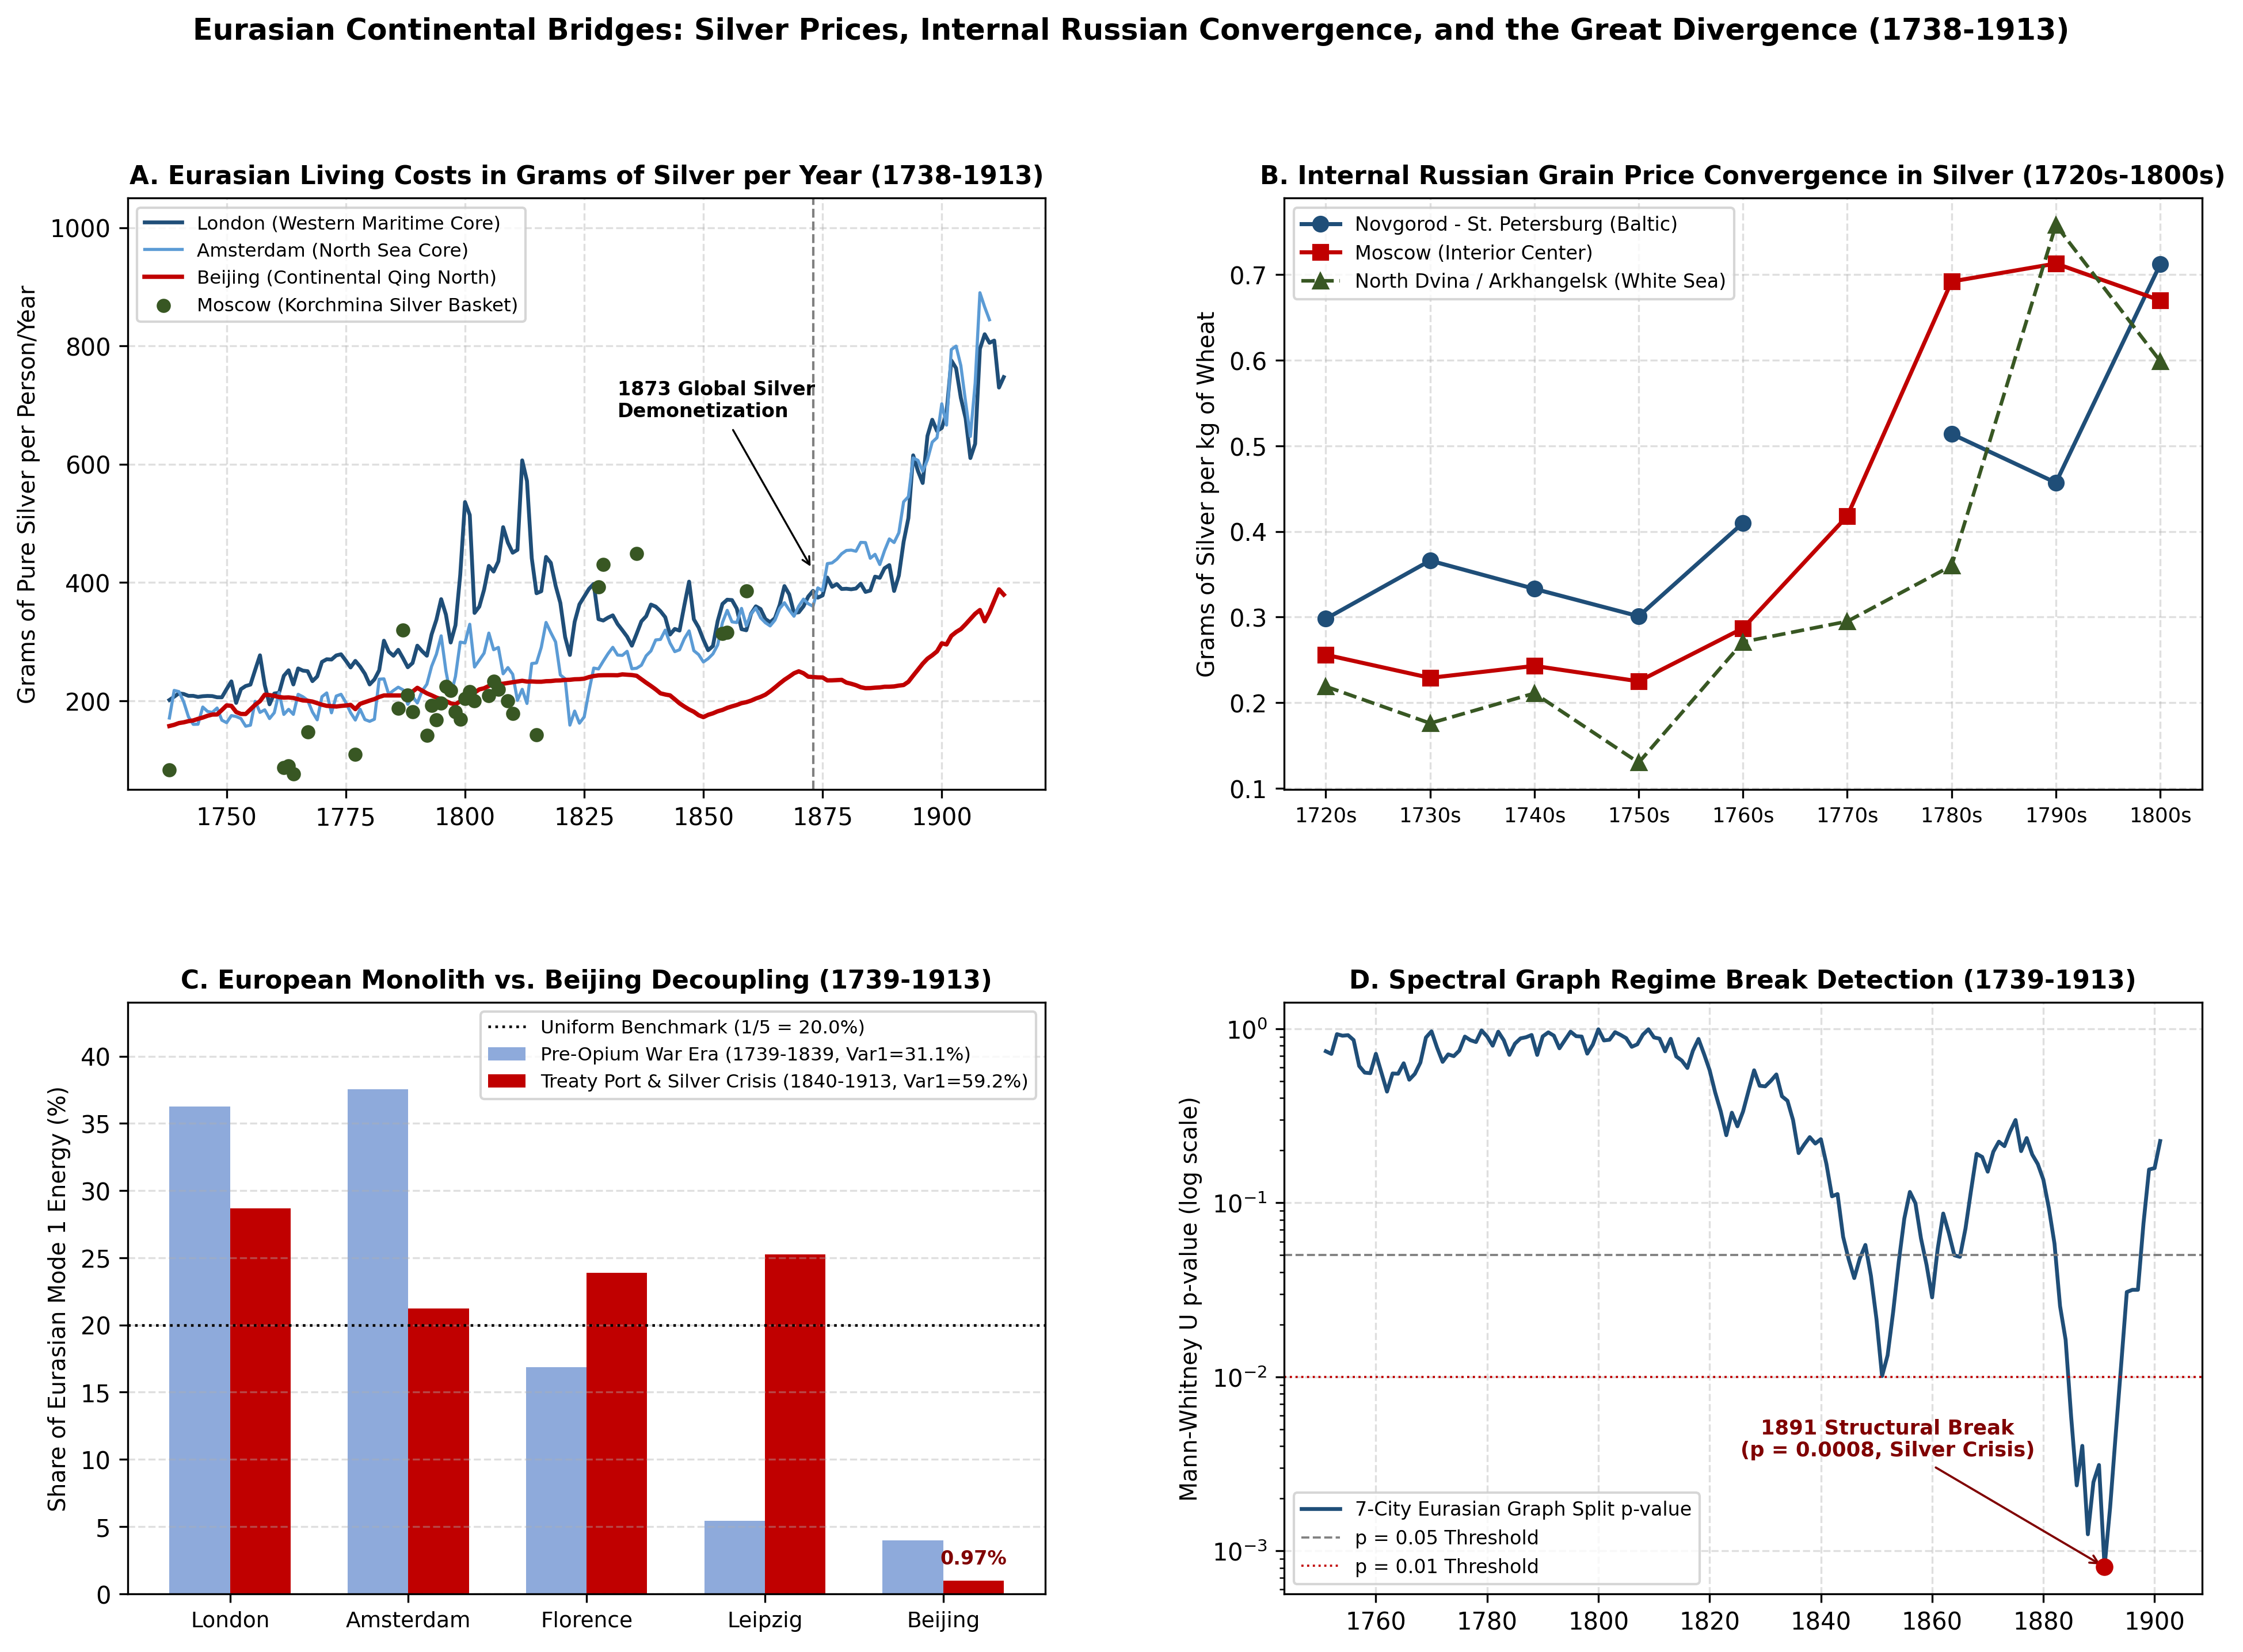
\includegraphics[width=\textwidth]{Figure_1_Eurasia.png}
\caption{\textbf{Eurasian Silver Living Costs, Internal Russian Convergence, and Regime Breaks (1738--1913).} \textbf{A:} Annual barebones subsistence basket costs (grams of pure silver per person-year) for London, Amsterdam, Beijing, and benchmark Moscow years. \textbf{B:} Decadal silver wheat prices across Novgorod--St.~Petersburg, Moscow, and North Dvina (Arkhangelsk), 1720s--1800s. \textbf{C:} Shift in Mode~1 variance shares before (1739--1839) and after (1840--1913) the Opium Wars. \textbf{D:} Non-parametric transition-graph scan ($p$-values on Fiedler vector $\psi_2$), identifying the 1891 silver-crisis structural break ($p = 0.0008$).}
\label{fig:fig1}
\end{figure}
Within Russia, early eighteenth-century grain prices displayed a steep coastal--interior gradient: in the 1730s--1750s, wheat in \texttt{Novgorod--St.~Petersburg} cost 0.30--0.37,g Ag/kg versus 0.23--0.24,g in \texttt{Moscow} and 0.13--0.21,g along the \texttt{North Dvina} (Figure~\ref{fig:fig1}B). Between 1760 and 1809, expanding domestic trade and urban demand pulled interior prices upward into convergence (0.67,g in Moscow, 0.71,g in St.~Petersburg, and 0.60,g in North Dvina), raising Moscow's silver subsistence basket from 100.1,g in the 1760s to 224.4,g in the 1780s—virtually identical to \texttt{Amsterdam} (207.9,g) and \texttt{Beijing} (208.0,g).
After 1873, however, global silver demonetization triggered a dramatic nominal divergence in silver-denominated living costs (Figure~\ref{fig:fig1}A). As gold-standard European economies absorbed rising silver-denominated price levels—reaching 713.6,g in London, 757.4,g in Amsterdam, 762.3,g in Leipzig, and 975.8,g in Florence by the 1900s—silver-standard \texttt{Beijing} remained anchored at 324.3,g Ag/year.
\subsection{Spectral Decomposition and the Two-Stage Eurasian Break (1857 vs.\ 1891)}
Applying singular value decomposition and transition-graph scanning (Appendix~A) to standardized annual log-changes $\Delta \ln \mathrm{CPI}_{t,j}$ quantifies the structural mechanics of the Eurasian divergence (Table~\ref{tab:eurasia_summary} and Figure~\ref{fig:fig1}C--D).
\begin{table}[htbp]
\centering
\caption{Spectral and Topological Summary of Eurasian Silver Price Integration (1739--1913)}
\label{tab:eurasia_summary}
\scriptsize
\setlength{\tabcolsep}{3pt}
\begin{tabular}{@{}p{0.27\textwidth}cccccc@{}}
\toprule
\textbf{Panel / Historical Era} & \textbf{Trans.} & \textbf{Mode 1} & \textbf{Mode 2} & \textbf{Temporal $\mathrm{PR}(u_1)$} & \textbf{Spatial $\mathrm{PR}(v_1)$} & \textbf{Graph Break ($p$)} \tabularnewline
\midrule
Unbroken 5-City CPI (1739--1913) & 175 & 35.6\% & 21.7\% & 0.264 [0.23, 0.31] & 0.668 [0.57, 0.75] & 1891 (0.0084) \tabularnewline
Uninterpolated 7-City CPI (1739--1833) & 95 & 24.2\% & 20.2\% & 0.352 [0.26, 0.39] & 0.647 [0.47, 0.76] & 1806 (0.1429) \tabularnewline
Bridged 7-City CPI (1739--1913) & 175 & 26.0\% & 20.6\% & 0.292 [0.24, 0.33] & 0.587 [0.45, 0.77] & 1891 (0.0008) \tabularnewline
Pre-Opium War CPI (1739--1839, $N=5$) & 101 & 31.1\% & 24.7\% & 0.262 [0.20, 0.38] & 0.569 [0.46, 0.74] & 1762 (0.3538) \tabularnewline
Treaty Port and Silver CPI (1840--1913, $N=5$) & 74 & 59.2\% & 20.1\% & 0.225 [0.19, 0.29] & 0.757 [0.72, 0.80] & 1899 (0.0737) \tabularnewline
5-City Welfare Ratios (1739--1913) & 175 & 31.2\% & 22.6\% & 0.265 [0.22, 0.31] & 0.601 [0.48, 0.75] & 1857 ($<$0.0001) \tabularnewline
\bottomrule
\end{tabular}
\vspace{1mm}
\begin{minipage}{\textwidth}
\footnotesize\emph{Notes:} Computed on standardized annual log-changes of barebones subsistence baskets in grams of pure silver (CPI) and real welfare ratios. Brackets report 95\% subsampling bootstrap confidence intervals (300 draws at 80\% sample length).
\end{minipage}
\end{table}


Comparing the pre-Opium War century (1739--1839) against the post-1840 treaty-port and silver-crisis era exposes two simultaneous transformations (Figure~\ref{fig:fig1}C):
\begin{itemize}
    \item \textbf{European Consolidation:} Between 1739--1839 and 1840--1913, shared Mode~1 variance across the five-city panel nearly doubled from 31.1\% to 59.2\%, while spatial participation climbed from $\mathrm{PR}(v_1) = 0.569$ to $0.757$. By 1840--1913, \texttt{London} (28.66\%), \texttt{Leipzig} (25.27\%), \texttt{Florence} (23.87\%), and \texttt{Amsterdam} (21.23\%) contributed almost identical shares to Mode~1, driven by synchronized European shocks in 1848 (12.6\% of Mode~1 energy), 1908 (12.5\%), and 1894 (9.2\%).
    \item \textbf{Continental Beijing Isolation:} Simultaneously, \texttt{Beijing}'s share of Mode~1 variance collapsed from 3.97\% before 1840 to just 0.97\% after 1840. In 1840--1913, 94.2\% of Beijing's variance was absorbed by orthogonal Mode~2 ($\mathrm{Var}_2 = 20.1\%$; $v_{2,\mathrm{Beijing}} = -0.971$), reflecting domestic Taiping-era monetary disruptions, copper-cash inflation, and Beijing's insulation from European gold-standard price dynamics.
\end{itemize}

Crucially, comparing transition-graph scans across nominal silver prices (CPI) and real living standards (welfare ratios) uncovers a two-stage Eurasian structural break (Table~\ref{tab:eurasia_summary} and Figure~\ref{fig:fig1}D): real welfare ratios fractured first in \texttt{1857} ($p < 0.0001$) amid the Taiping Rebellion, the Second Opium War, and mid-century industrial divergence, whereas silver-denominated price levels broke decisively in \texttt{1891} ($p = 0.0084$ in the five-city panel and $p = 0.0008$ in the seven-city panel), when global silver demonetization severed the eighteenth-century metallic price corridor.

\subsection{Tri-Polar Eurasia: Uninterpolated Validation and Welfare Divergence}
To verify that the three-way division of Eurasia is not an artifact of post-1834 reporting gaps in southern China, we inspect the strictly uninterpolated seven-city panel over \texttt{1739--1833} ($M = 95$, zero missing values) alongside the full 1739--1913 projection (Figure~\ref{fig:fig2}A). Even before the Opium Wars, the uninterpolated loadings divide Eurasia into three distinct poles:
\begin{enumerate}
    \item \textbf{The Western/Central European Core} (\texttt{Amsterdam} $v_1 = +0.553$, \texttt{London} $+0.464$, \texttt{Leipzig} $+0.357$, \texttt{Florence} $+0.262$) co-moves positively along Mode~1 ($\mathrm{Var}_1 = 24.2\%$).
    \item \textbf{Maritime Southern China} (\texttt{Canton} $v_1 = -0.436$, \texttt{Suzhou} $v_1 = -0.298$) loads negatively on Mode~1, moving counter-cyclically to European bullion and grain fluctuations.
    \item \textbf{Continental Northern China} (\texttt{Beijing}, the terminus of the overland Siberian--Kyakhta caravan trade) exhibits near-zero loading on Mode~1 ($v_1 = +0.066$, accounting for just 0.43\% of Mode~1 energy) and sits on orthogonal Mode~2 ($v_2 = +0.451$; $\mathrm{Var}_2 = 20.2\%$), confirming that northern continental China operated independently of both European and maritime coastal Chinese price cycles.
\end{enumerate}

\begin{figure}[htbp]
\centering
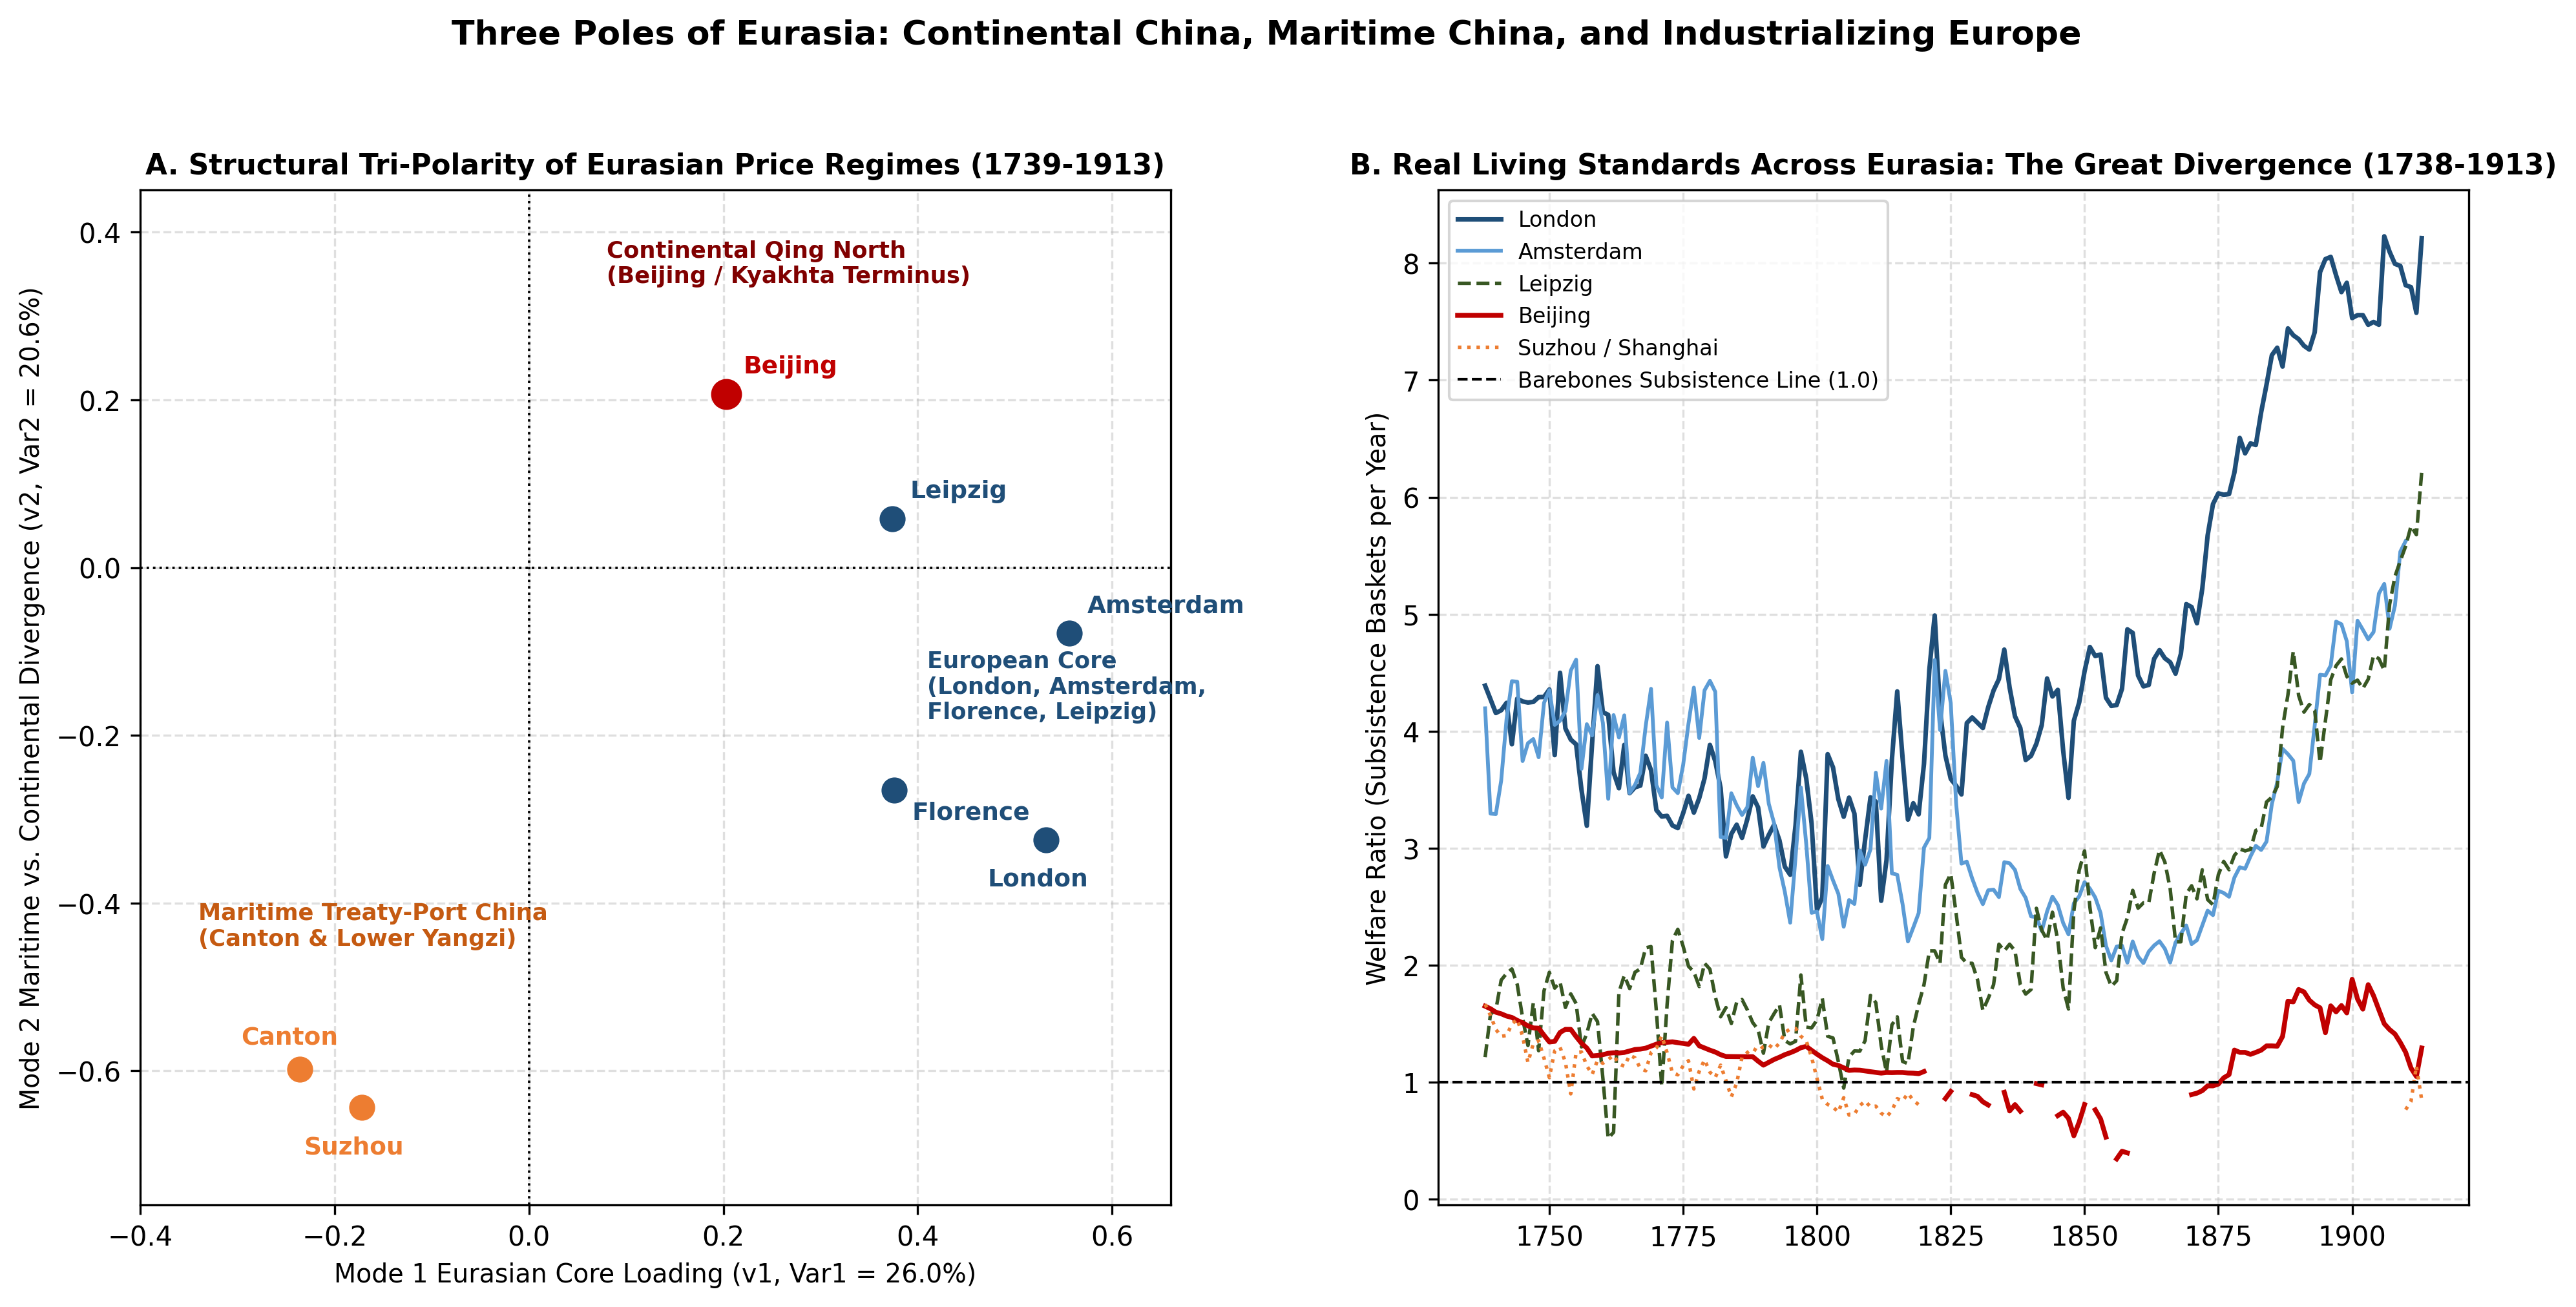
\includegraphics[width=\textwidth]{Figure_2_Eurasia.png}
\caption{\textbf{Tri-Polar Eurasian Price Structure and Welfare Ratio Divergence (1738--1913).} \textbf{A:} Two-mode spectral map of seven Eurasian cities (1739--1913), separating the European core from continental Beijing and maritime Canton/Suzhou. \textbf{B:} Real living standards (welfare ratios, defined as annual unskilled earnings divided by barebones subsistence basket cost) across London, Amsterdam, Leipzig, Beijing, and Suzhou/Shanghai (1738--1913).}
\label{fig:fig2}
\end{figure}

This structural divergence in silver prices directly mirrors the divergence in real living standards (Figure~\ref{fig:fig2}B). While welfare ratios in \texttt{Beijing} and \texttt{Suzhou/Shanghai} hovered near or slightly above the barebones subsistence threshold ($1.0\text{--}1.8$ baskets per year) from the 1740s through 1913—dipping below $1.0$ during mid-nineteenth-century crises—industrializing \texttt{London} and \texttt{Amsterdam} broke away after the 1820s, rising from $3\text{--}4$ subsistence baskets to $6\text{--}8$ baskets per year by 1913.

\section{Discussion and Conclusion}

Synthesizing all four studies in our empirical cycle yields a unified map of how Eurasia's regional economies connected—and fractured—between the eighteenth and early twentieth centuries. In the West, St.~Petersburg and European Russia integrated sequentially with Europe: first in physical Baltic commodity flows after 1721 (\href{https://doi.org}{Avtonomov, 2026b}), next in internal grain price convergence and Atlantic food arbitrage during the nineteenth century (\href{https://doi.org}{Avtonomov, 2026a}), and finally in foreign exchange synchronization following Kankrin's 1839 silver reform and Witte's 1897 gold standard (\href{https://doi.org}{Avtonomov, 2026c}).

Looking eastward across the Eurasian continent reveals the mirror image of that integration. While eighteenth-century Eurasia shared a common silver price corridor from London through Moscow to Beijing, the nineteenth century produced a two-stage divergence: real welfare ratios split first in \texttt{1857} ($p < 0.0001$), followed by a monetary price break in \texttt{1891} ($p = 0.0008$) as Western Europe consolidated into a synchronized gold-standard block ($\mathrm{Var}_1 = 59.2\%$) while continental Qing China remained anchored to an isolated silver regime (Mode~1 share = 0.97\%). Across every geographic scale—from Baltic ports to the Kyakhta--Beijing continental axis—historical market integration was governed by the alignment of monetary standards and transport infrastructure rather than automatic price equalization.

\section*{Data and Code Availability}
All underlying datasets are openly available from the Global Price and Income History Group (\url{ucdavis.edu}: Allen et al., 2011; Korchmina, 2025; Mironov, 2010). Reproducible Python/Jupyter code, high-resolution figures, and LaTeX manuscript sources are archived at \url{github.com/avtonomov-petr/Eurosean-Continental-Bridges}.
\appendix
\section{Mathematical Specification of Diagnostics}
Let $C_{t,j} > 0$ denote the annual barebones subsistence basket cost (or real welfare ratio) of city $j \in \{1,\dots,N\}$ in year $t$. Annual log-changes $y_{t,j} = \ln C_{t,j} - \ln C_{t-1,j}$ across $M$ transitions are standardized to zero mean and unit variance, $Z_{t,j} = (y_{t,j} - \bar{y}_j)/s_j$. Thin singular value decomposition $Z = U \Sigma V^\top$ yields temporal scores $u_k \in \mathbb{R}^M$ and spatial loadings $v_k \in \mathbb{R}^N$, with normalized participation ratios:
\begin{equation}
\mathrm{PR}(u_1) = \frac{\left(\sum_{t=1}^M u_{t,1}^4\right)^{-1} - 1}{M - 1}, \qquad
\mathrm{PR}(v_1) = \frac{\left(\sum_{j=1}^N v_{j,1}^4\right)^{-1} - 1}{N - 1}.
\end{equation}
Structural regime breaks are evaluated on a symmetric $k$-nearest-neighbor Gaussian affinity graph ($k=6$, calibrated to compact cross-sectional panels $N \in \{5,7\}$; bandwidth $\sigma$ equal to the median pairwise Euclidean distance) by scanning two-sided Mann--Whitney $U$ tests along the Fiedler eigenvector $\psi_2$ of $L_{\mathrm{sym}} = I - D^{-1/2} A D^{-1/2}$ for candidate split years $\tau \in [12, M-12]$.

\begin{thebibliography}{99}
\bibitem{Allen2011}
Allen, R. C., Bassino, J.-P., Ma, D., Moll-Murata, C., \& van Zanden, J. L. (2011). Wages, prices, and living standards in China, 1738--1925: In comparison with Europe, Japan, and India. \emph{Economic History Review}, 64(S1), 8--38.
\bibitem{Avtonomov2026a}
Avtonomov, P. (2026a). Crisis echoes or arbitrage? Selective co-movement and integration of the Atlantic grain market, 1729--1914. \emph{Zenodo Preprint}. \url{https://doi.org/10.5281/zenodo.24436177}
\bibitem{Avtonomov2026b}
Avtonomov, P. (2026b). Blockades, flag mimicry, and grain lifelines: Physical anatomy of Russian and Baltic maritime trade in the Sound Toll Registers, 1700--1856. \emph{Zenodo Preprint}. \url{https://doi.org/10.5281/zenodo.24461586}
\bibitem{Avtonomov2026c}
Avtonomov, P. (2026c). Invisible bridges of credit: Exchange rate integration, paper assignats, and metallic anchors between St.~Petersburg and Europe, 1763--1913. \emph{Zenodo Preprint}. \url{https://doi.org/10.5281/zenodo.24498028}
\bibitem{Broadberry2018}
Broadberry, S., Guan, H., \& Li, D. D. (2018). China, Europe, and the Great Divergence: A study in historical national accounting, 980--1850. \emph{Journal of Economic History}, 78(4), 955--1000.
\bibitem{Foust1969}
Foust, C. M. (1969). \emph{Muscovite and Mandarin: Russia's trade with China and its setting, 1727--1805}. University of North Carolina Press.
\bibitem{Korchmina2025}
Korchmina, E. (2025). Moscow living standards and silver subsistence baskets, 1706--1860. \emph{Global Price and Income History Group Dataset}, UC Davis.
\bibitem{Mironov2010}
Mironov, B. N. (2010). \emph{Blagosostoianie naseleniia i revoliutsii v imperskoi Rossii: XVIII -- nachalo XX veka} [Living standards and revolutions in Imperial Russia, 18th -- early 20th centuries]. Novyi Khronograf.
\bibitem{Pomeranz2000}
Pomeranz, K. (2000). \emph{The Great Divergence: China, Europe, and the making of the modern world economy}. Princeton University Press.
\bibitem{Sladkovskii1974}
Sladkovskii, M. I. (1974). \emph{Istoriia torgovo-ekonomicheskikh otnoshenii narodov Rossii s Kitaem (do 1917 g.)} [History of trade and economic relations of the peoples of Russia with China before 1917]. Nauka.
\end{thebibliography}
\section*{Figure Alt Text}
\begin{itemize}
\item \textbf{Figure 1 Alt Text:} Four-panel chart of Eurasian silver living costs, internal Russian decadal wheat prices, pre- and post-1840 Mode~1 variance shares, and graph transition p-values showing an 1891 structural break.
\item \textbf{Figure 2 Alt Text:} Scatter plot of seven Eurasian cities across Modes~1 and~2 and time series of real welfare ratios across London, Amsterdam, Leipzig, Beijing, and Suzhou/Shanghai from 1738 to 1913.
\end{itemize}
\end{document}